\documentclass[a4paper]{book}
\usepackage{a4wide}
\usepackage{makeidx}
\usepackage{fancyhdr}
\usepackage{graphicx}
\usepackage{multicol}
\usepackage{float}
\usepackage{textcomp}
\usepackage{alltt}
\usepackage{times}
\usepackage{ifpdf}
\ifpdf
\usepackage[pdftex,
            pagebackref=true,
            colorlinks=true,
            linkcolor=blue,
            unicode
           ]{hyperref}
\else
\usepackage[ps2pdf,
            pagebackref=true,
            colorlinks=true,
            linkcolor=blue,
            unicode
           ]{hyperref}
\usepackage{pspicture}
\fi
\usepackage[utf8]{inputenc}
\usepackage{doxygen}
\makeindex
\setcounter{tocdepth}{3}
\renewcommand{\footrulewidth}{0.4pt}
\begin{document}
\begin{titlepage}
\vspace*{7cm}
\begin{center}
{\Large lighttpd-cpp }\\
\vspace*{1cm}
{\large Generated by Doxygen 1.5.8}\\
\vspace*{0.5cm}
{\small Sat Jul 18 21:16:55 2009}\\
\end{center}
\end{titlepage}
\clearemptydoublepage
\pagenumbering{roman}
\tableofcontents
\clearemptydoublepage
\pagenumbering{arabic}
\chapter{Class Index}
\section{Class Hierarchy}
This inheritance list is sorted roughly, but not completely, alphabetically:\begin{CompactList}
\item \contentsline{section}{\_\-fdnode}{\pageref{struct__fdnode}}{}
\item \contentsline{section}{ajp13\_\-state\_\-data}{\pageref{structajp13__state__data}}{}
\item \contentsline{section}{config\_\-option\_\-base}{\pageref{structconfig__option__base}}{}
\item \contentsline{section}{connection\_\-map\_\-entry}{\pageref{structconnection__map__entry}}{}
\item \contentsline{section}{errorlog}{\pageref{structerrorlog}}{}
\item \contentsline{section}{excludes}{\pageref{structexcludes}}{}
\item \contentsline{section}{fcgi\_\-state\_\-data}{\pageref{structfcgi__state__data}}{}
\item \contentsline{section}{fd\_\-conn}{\pageref{structfd__conn}}{}
\item \contentsline{section}{fdevent\_\-revent}{\pageref{structfdevent__revent}}{}
\item \contentsline{section}{fdevents}{\pageref{structfdevents}}{}
\item \contentsline{section}{handlers\_\-setter\_\-base$<$ PluginType, HandlerList $>$}{\pageref{structhandlers__setter__base}}{}
\begin{CompactList}
\item \contentsline{section}{handlers\_\-setter\_\-impl$<$ PluginType, Handler, HandlerList $>$}{\pageref{structhandlers__setter__impl}}{}
\end{CompactList}
\item \contentsline{section}{handlers\_\-setter\_\-end}{\pageref{structhandlers__setter__end}}{}
\item \contentsline{section}{iosocket}{\pageref{structiosocket}}{}
\item \contentsline{section}{plugin}{\pageref{structplugin}}{}
\item \contentsline{section}{plugin\_\-base}{\pageref{classplugin__base}}{}
\begin{CompactList}
\item \contentsline{section}{Plugin$<$ MostDerived $>$}{\pageref{classPlugin}}{}
\end{CompactList}
\item \contentsline{section}{plugin\_\-config}{\pageref{structplugin__config}}{}
\item \contentsline{section}{protocol\_\-state\_\-data}{\pageref{structprotocol__state__data}}{}
\item \contentsline{section}{proxy\_\-backlog}{\pageref{structproxy__backlog}}{}
\item \contentsline{section}{proxy\_\-connection}{\pageref{structproxy__connection}}{}
\end{CompactList}

\chapter{Class Index}
\section{Class List}
Here are the classes, structs, unions and interfaces with brief descriptions:\begin{CompactList}
\item\contentsline{section}{\hyperlink{struct__fdnode}{\_\-fdnode} }{\pageref{struct__fdnode}}{}
\item\contentsline{section}{\hyperlink{structajp13__state__data}{ajp13\_\-state\_\-data} }{\pageref{structajp13__state__data}}{}
\item\contentsline{section}{\hyperlink{structconfig__option__base}{config\_\-option\_\-base} }{\pageref{structconfig__option__base}}{}
\item\contentsline{section}{\hyperlink{structconnection__map__entry}{connection\_\-map\_\-entry} }{\pageref{structconnection__map__entry}}{}
\item\contentsline{section}{\hyperlink{structerrorlog}{errorlog} }{\pageref{structerrorlog}}{}
\item\contentsline{section}{\hyperlink{structexcludes}{excludes} }{\pageref{structexcludes}}{}
\item\contentsline{section}{\hyperlink{structfcgi__state__data}{fcgi\_\-state\_\-data} }{\pageref{structfcgi__state__data}}{}
\item\contentsline{section}{\hyperlink{structfd__conn}{fd\_\-conn} }{\pageref{structfd__conn}}{}
\item\contentsline{section}{\hyperlink{structfdevent__revent}{fdevent\_\-revent} }{\pageref{structfdevent__revent}}{}
\item\contentsline{section}{\hyperlink{structfdevents}{fdevents} }{\pageref{structfdevents}}{}
\item\contentsline{section}{\hyperlink{structhandlers__setter__base}{handlers\_\-setter\_\-base$<$ PluginType, HandlerList $>$} }{\pageref{structhandlers__setter__base}}{}
\item\contentsline{section}{\hyperlink{structhandlers__setter__end}{handlers\_\-setter\_\-end} }{\pageref{structhandlers__setter__end}}{}
\item\contentsline{section}{\hyperlink{structhandlers__setter__impl}{handlers\_\-setter\_\-impl$<$ PluginType, Handler, HandlerList $>$} }{\pageref{structhandlers__setter__impl}}{}
\item\contentsline{section}{\hyperlink{structiosocket}{iosocket} }{\pageref{structiosocket}}{}
\item\contentsline{section}{\hyperlink{structplugin}{plugin} }{\pageref{structplugin}}{}
\item\contentsline{section}{\hyperlink{classPlugin}{Plugin$<$ MostDerived $>$} }{\pageref{classPlugin}}{}
\item\contentsline{section}{\hyperlink{classplugin__base}{plugin\_\-base} }{\pageref{classplugin__base}}{}
\item\contentsline{section}{\hyperlink{structplugin__config}{plugin\_\-config} }{\pageref{structplugin__config}}{}
\item\contentsline{section}{\hyperlink{structprotocol__state__data}{protocol\_\-state\_\-data} }{\pageref{structprotocol__state__data}}{}
\item\contentsline{section}{\hyperlink{structproxy__backlog}{proxy\_\-backlog} }{\pageref{structproxy__backlog}}{}
\item\contentsline{section}{\hyperlink{structproxy__connection}{proxy\_\-connection} }{\pageref{structproxy__connection}}{}
\end{CompactList}

\chapter{Class Documentation}
\hypertarget{struct__fdnode}{
\section{\_\-fdnode Struct Reference}
\label{struct__fdnode}\index{\_\-fdnode@{\_\-fdnode}}
}
{\tt \#include $<$fdevent.h$>$}

\subsection*{Public Attributes}
\begin{CompactItemize}
\item 
\hypertarget{struct__fdnode_197ee75ecdf4018d2b6eec823dc67ff4}{
fdevent\_\-handler \textbf{handler}}
\label{struct__fdnode_197ee75ecdf4018d2b6eec823dc67ff4}

\item 
\hypertarget{struct__fdnode_b89a325bfe82c899da15e739a15925b4}{
void $\ast$ \textbf{ctx}}
\label{struct__fdnode_b89a325bfe82c899da15e739a15925b4}

\item 
\hypertarget{struct__fdnode_00a11f60bb26e73cb7fb6e84bb4ffbc4}{
int \textbf{fd}}
\label{struct__fdnode_00a11f60bb26e73cb7fb6e84bb4ffbc4}

\item 
\hypertarget{struct__fdnode_67eb5eaee2c2e43654d70954da4ce6cc}{
struct \hyperlink{struct__fdnode}{\_\-fdnode} $\ast$ \textbf{prev}}
\label{struct__fdnode_67eb5eaee2c2e43654d70954da4ce6cc}

\item 
\hypertarget{struct__fdnode_d6809dc25a8f98514886f9a2fea86a54}{
struct \hyperlink{struct__fdnode}{\_\-fdnode} $\ast$ \textbf{next}}
\label{struct__fdnode_d6809dc25a8f98514886f9a2fea86a54}

\end{CompactItemize}


\subsection{Detailed Description}
array of unused fd's 

The documentation for this struct was generated from the following file:\begin{CompactItemize}
\item 
include/lighttpd/fdevent.h\end{CompactItemize}

\hypertarget{structajp13__state__data}{
\section{ajp13\_\-state\_\-data Struct Reference}
\label{structajp13__state__data}\index{ajp13\_\-state\_\-data@{ajp13\_\-state\_\-data}}
}
\subsection*{Public Attributes}
\begin{CompactItemize}
\item 
\hypertarget{structajp13__state__data_05104320fc4dfebffd6e199c2a1cf223}{
buffer $\ast$ \textbf{buf}}
\label{structajp13__state__data_05104320fc4dfebffd6e199c2a1cf223}

\item 
\hypertarget{structajp13__state__data_15408e96744b63ad6cd03e83ff6e1369}{
off\_\-t \textbf{offset}}
\label{structajp13__state__data_15408e96744b63ad6cd03e83ff6e1369}

\item 
\hypertarget{structajp13__state__data_66198f3c961de2525eeb5c63171ffb13}{
ajp13\_\-packet \textbf{packet}}
\label{structajp13__state__data_66198f3c961de2525eeb5c63171ffb13}

\item 
\hypertarget{structajp13__state__data_1931c23e738ac24b5797ccaa5a5a875e}{
size\_\-t \textbf{chunk\_\-len}}
\label{structajp13__state__data_1931c23e738ac24b5797ccaa5a5a875e}

\item 
\hypertarget{structajp13__state__data_8487799ea44d1f053807646845a9d617}{
size\_\-t \textbf{requested\_\-bytes}}
\label{structajp13__state__data_8487799ea44d1f053807646845a9d617}

\end{CompactItemize}


\subsection{Detailed Description}
The ajp13 protocol decoder will use this struct for storing state variables used in decoding the stream 

The documentation for this struct was generated from the following file:\begin{CompactItemize}
\item 
include/lighttpd/mod\_\-proxy\_\-backend\_\-ajp13.c\end{CompactItemize}

\hypertarget{structconfig__option__base}{
\section{config\_\-option\_\-base Struct Reference}
\label{structconfig__option__base}\index{config\_\-option\_\-base@{config\_\-option\_\-base}}
}
{\tt \#include $<$datatype\_\-helpers.hpp$>$}

Inherited by config\_\-option$<$ OptionType, ConfigScopeType, OptionTraits $>$.

\subsection*{Public Types}
\begin{CompactItemize}
\item 
\hypertarget{structconfig__option__base_b71046712f2629513bf074eb030dc3b7}{
typedef std::vector$<$ \hyperlink{structconfig__option__base}{config\_\-option\_\-base} $\ast$ $>$ \textbf{registry\_\-type}}
\label{structconfig__option__base_b71046712f2629513bf074eb030dc3b7}

\item 
\hypertarget{structconfig__option__base_23ce095890ffe80c8bc31f7cb90d3f4f}{
typedef registry\_\-type::iterator \textbf{registry\_\-iterator}}
\label{structconfig__option__base_23ce095890ffe80c8bc31f7cb90d3f4f}

\item 
\hypertarget{structconfig__option__base_badbd3acf8284e0cdb3a0e637498c6e7}{
typedef registry\_\-type::const\_\-iterator \textbf{registry\_\-const\_\-iterator}}
\label{structconfig__option__base_badbd3acf8284e0cdb3a0e637498c6e7}

\end{CompactItemize}
\subsection*{Public Member Functions}
\begin{CompactItemize}
\item 
\hypertarget{structconfig__option__base_5f87eab8c0be092869b305fd1ef3f133}{
\textbf{config\_\-option\_\-base} (const char $\ast$key)}
\label{structconfig__option__base_5f87eab8c0be092869b305fd1ef3f133}

\item 
\hypertarget{structconfig__option__base_ac53aa895594570d1707c302909d266c}{
virtual handler\_\-t \textbf{set\_\-defaults} (const server \&srv)=0}
\label{structconfig__option__base_ac53aa895594570d1707c302909d266c}

\item 
\hypertarget{structconfig__option__base_c2eb1e7e5bbc509803cd19ffeeda331e}{
virtual handler\_\-t \textbf{set\_\-defaults} ()=0}
\label{structconfig__option__base_c2eb1e7e5bbc509803cd19ffeeda331e}

\end{CompactItemize}
\subsection*{Static Public Member Functions}
\begin{CompactItemize}
\item 
\hypertarget{structconfig__option__base_1a33ba2de88522286bad68735ae9bb0e}{
static handler\_\-t \textbf{set\_\-all\_\-defaults} ()}
\label{structconfig__option__base_1a33ba2de88522286bad68735ae9bb0e}

\end{CompactItemize}
\subsection*{Public Attributes}
\begin{CompactItemize}
\item 
\hypertarget{structconfig__option__base_9e1952a48dc047f2e2152b767e9d0c65}{
const char $\ast$ \textbf{key}}
\label{structconfig__option__base_9e1952a48dc047f2e2152b767e9d0c65}

\item 
\hypertarget{structconfig__option__base_700ece40b8a2feb8f1b8c9196660ade0}{
const server $\ast$ \textbf{srv}}
\label{structconfig__option__base_700ece40b8a2feb8f1b8c9196660ade0}

\end{CompactItemize}
\subsection*{Static Public Attributes}
\begin{CompactItemize}
\item 
\hypertarget{structconfig__option__base_0fcfa3fa7ba3396e7dfb1b9d27970592}{
static registry\_\-type \textbf{registry}}
\label{structconfig__option__base_0fcfa3fa7ba3396e7dfb1b9d27970592}

\end{CompactItemize}


\subsection{Detailed Description}
These are classes to automate the filling of what would be the \hyperlink{structplugin__config}{plugin\_\-config} and plugin\_\-data structures if we were using C, making the following valid (or close to valid): struct mod\_\-blank \{ mod\_\-blank( ... ) : hostname( \char`\"{}some-config-tag\char`\"{} \mbox{[}, \&validator \mbox{[}, \&default\_\-setter\mbox{]} \mbox{]} ) \{ ... \} std::string\& default\_\-setter( std::string\& s )\{ ... return std::string( \char`\"{}asdf\char`\"{} ); \} config\_\-option$<$ std::string $>$ hostname; \};

So a config options type is specified at runtime, and we can add new types sit on top of the lighttpd ones. i.e. we could have a network mask type, getting options from T\_\-CONFIG\_\-STRING and that checks for the correct formatting. If incorrect we could throw an exception to be caught by the set\_\-defaults handler, or we could set it to the value returned by default\_\-setter. 

The documentation for this struct was generated from the following file:\begin{CompactItemize}
\item 
include/lighttpd-cpp/datatype\_\-helpers.hpp\end{CompactItemize}

\hypertarget{structconnection__map__entry}{
\section{connection\_\-map\_\-entry Struct Reference}
\label{structconnection__map__entry}\index{connection\_\-map\_\-entry@{connection\_\-map\_\-entry}}
}
\subsection*{Public Attributes}
\begin{CompactItemize}
\item 
\hypertarget{structconnection__map__entry_9b850dc1eeab1d8c44db1ce3d5dd0365}{
buffer $\ast$ \textbf{tracking\_\-id}}
\label{structconnection__map__entry_9b850dc1eeab1d8c44db1ce3d5dd0365}

\item 
\hypertarget{structconnection__map__entry_32512220136d43a40f2219f87b9689ee}{
connection $\ast$ \textbf{con}}
\label{structconnection__map__entry_32512220136d43a40f2219f87b9689ee}

\item 
\hypertarget{structconnection__map__entry_97413e3f9c37b9d35c0cce27cb68aa2d}{
time\_\-t \textbf{timeout}}
\label{structconnection__map__entry_97413e3f9c37b9d35c0cce27cb68aa2d}

\item 
\hypertarget{structconnection__map__entry_a2c3e39ece01ae70c3edabff7d98ccd5}{
int \textbf{status}}
\label{structconnection__map__entry_a2c3e39ece01ae70c3edabff7d98ccd5}

\item 
\hypertarget{structconnection__map__entry_6c982b1a4aa90aed9e69d2f0504630d5}{
off\_\-t \textbf{size}}
\label{structconnection__map__entry_6c982b1a4aa90aed9e69d2f0504630d5}

\end{CompactItemize}


\subsection{Detailed Description}
uploadprogress for lighttpd

Initial: Jan Kneschke $<$\href{mailto:jan@kneschke.de}{\tt jan@kneschke.de}$>$ Timeout+Status addon: Bjoern Kalkbrenner $<$\href{mailto:terminar@cyberphoria.org}{\tt terminar@cyberphoria.org}$>$ \mbox{[}20070112\mbox{]}

the timeout is used to keep in the status information intact even if the parent connection is gone already 

The documentation for this struct was generated from the following file:\begin{CompactItemize}
\item 
include/lighttpd/mod\_\-uploadprogress.c\end{CompactItemize}

\hypertarget{structerrorlog}{
\section{errorlog Struct Reference}
\label{structerrorlog}\index{errorlog@{errorlog}}
}
\subsection*{Public Types}
\begin{CompactItemize}
\item 
enum \{ \textbf{ERRORLOG\_\-FILE}, 
\textbf{ERRORLOG\_\-FD}, 
\textbf{ERRORLOG\_\-SYSLOG}
 \}
\subsection*{Public Attributes}
\begin{CompactItemize}
\item 
\hypertarget{structerrorlog_91c64c945bcc42d0c568986ebc56aec6}{
buffer $\ast$ \textbf{file}}
\label{structerrorlog_91c64c945bcc42d0c568986ebc56aec6}

\item 
\hypertarget{structerrorlog_819e991bf71f814ce719f2bbc54f0c3c}{
unsigned short \textbf{use\_\-syslog}}
\label{structerrorlog_819e991bf71f814ce719f2bbc54f0c3c}

\item 
\hypertarget{structerrorlog_7c742fe7ce6efd7d689e4be156ba5a03}{
int \textbf{fd}}
\label{structerrorlog_7c742fe7ce6efd7d689e4be156ba5a03}

\item 
\hypertarget{structerrorlog_d8f03d4f8a50455a5e008da0e3e491db}{
enum errorlog:: \{ ... \}  \textbf{mode}}
\label{structerrorlog_d8f03d4f8a50455a5e008da0e3e491db}

\item 
\hypertarget{structerrorlog_6c5005571427e17c515dd26844db1ea1}{
buffer $\ast$ \textbf{buf}}
\label{structerrorlog_6c5005571427e17c515dd26844db1ea1}

\item 
\hypertarget{structerrorlog_79fa384854edf62041ab26fd07cde87b}{
time\_\-t \textbf{cached\_\-ts}}
\label{structerrorlog_79fa384854edf62041ab26fd07cde87b}

\item 
\hypertarget{structerrorlog_567be0d81abbaf275cb070b980855f47}{
buffer $\ast$ \textbf{cached\_\-ts\_\-str}}
\label{structerrorlog_567be0d81abbaf275cb070b980855f47}

\end{CompactItemize}


\subsection{Detailed Description}
open the \hyperlink{structerrorlog}{errorlog}

we have 3 possibilities:\begin{itemize}
\item stderr (default)\item syslog\item logfile\end{itemize}


if the open failed, report to the user and die 

The documentation for this struct was generated from the following file:\begin{CompactItemize}
\item 
include/lighttpd/log.c\end{CompactItemize}

\hypertarget{structexcludes}{
\section{excludes Struct Reference}
\label{structexcludes}\index{excludes@{excludes}}
}
\subsection*{Public Attributes}
\begin{CompactItemize}
\item 
\hypertarget{structexcludes_ad6f3586601eba5c68854a77630abee2}{
buffer $\ast$ \textbf{string}}
\label{structexcludes_ad6f3586601eba5c68854a77630abee2}

\end{CompactItemize}


\subsection{Detailed Description}
this is a dirlisting for a lighttpd \hyperlink{structplugin}{plugin} 

The documentation for this struct was generated from the following file:\begin{CompactItemize}
\item 
include/lighttpd/mod\_\-dirlisting.c\end{CompactItemize}

\hypertarget{structfcgi__state__data}{
\section{fcgi\_\-state\_\-data Struct Reference}
\label{structfcgi__state__data}\index{fcgi\_\-state\_\-data@{fcgi\_\-state\_\-data}}
}
\subsection*{Public Attributes}
\begin{CompactItemize}
\item 
\hypertarget{structfcgi__state__data_1c08998287de5b4100c2728bb5afa817}{
buffer $\ast$ \textbf{buf}}
\label{structfcgi__state__data_1c08998287de5b4100c2728bb5afa817}

\item 
\hypertarget{structfcgi__state__data_11e9687ecbf38c3b6546169580ec89ba}{
fastcgi\_\-packet \textbf{packet}}
\label{structfcgi__state__data_11e9687ecbf38c3b6546169580ec89ba}

\item 
\hypertarget{structfcgi__state__data_c4b596fcc3f555b84cb215e2190aeed0}{
int \textbf{is\_\-complete}}
\label{structfcgi__state__data_c4b596fcc3f555b84cb215e2190aeed0}

\end{CompactItemize}


\subsection{Detailed Description}
The fastcgi protocol decoder will use this struct for storing state variables used in decoding the stream 

The documentation for this struct was generated from the following file:\begin{CompactItemize}
\item 
include/lighttpd/mod\_\-proxy\_\-backend\_\-fastcgi.c\end{CompactItemize}

\hypertarget{structfd__conn}{
\section{fd\_\-conn Struct Reference}
\label{structfd__conn}\index{fd\_\-conn@{fd\_\-conn}}
}
{\tt \#include $<$fdevent.h$>$}

\subsection*{Public Attributes}
\begin{CompactItemize}
\item 
int \hyperlink{structfd__conn_576721c825a9faed73f007b6a9ed8d5f}{fd}
\item 
void $\ast$ \hyperlink{structfd__conn_def788a594e0605705bcba2b45f7d454}{conn}
\item 
fd\_\-event\_\-t \hyperlink{structfd__conn_17c1513ada1c24eddf52b5e4654452d5}{fd\_\-type}
\item 
int \hyperlink{structfd__conn_a83443abeee1a38a020988475e2ea768}{events}
\item 
\hypertarget{structfd__conn_d668589ad75f5957b1b860e5609856d5}{
int \textbf{revents}}
\label{structfd__conn_d668589ad75f5957b1b860e5609856d5}

\end{CompactItemize}


\subsection{Detailed Description}
a mapping from fd to connection structure 

\subsection{Member Data Documentation}
\hypertarget{structfd__conn_def788a594e0605705bcba2b45f7d454}{
\index{fd\_\-conn@{fd\_\-conn}!conn@{conn}}
\index{conn@{conn}!fd_conn@{fd\_\-conn}}
\subsubsection[{conn}]{\setlength{\rightskip}{0pt plus 5cm}void$\ast$ {\bf fd\_\-conn::conn}}}
\label{structfd__conn_def788a594e0605705bcba2b45f7d454}


a reference the corresponding data-structure \hypertarget{structfd__conn_a83443abeee1a38a020988475e2ea768}{
\index{fd\_\-conn@{fd\_\-conn}!events@{events}}
\index{events@{events}!fd_conn@{fd\_\-conn}}
\subsubsection[{events}]{\setlength{\rightskip}{0pt plus 5cm}int {\bf fd\_\-conn::events}}}
\label{structfd__conn_a83443abeee1a38a020988475e2ea768}


registered events \hypertarget{structfd__conn_576721c825a9faed73f007b6a9ed8d5f}{
\index{fd\_\-conn@{fd\_\-conn}!fd@{fd}}
\index{fd@{fd}!fd_conn@{fd\_\-conn}}
\subsubsection[{fd}]{\setlength{\rightskip}{0pt plus 5cm}int {\bf fd\_\-conn::fd}}}
\label{structfd__conn_576721c825a9faed73f007b6a9ed8d5f}


the fd \hypertarget{structfd__conn_17c1513ada1c24eddf52b5e4654452d5}{
\index{fd\_\-conn@{fd\_\-conn}!fd\_\-type@{fd\_\-type}}
\index{fd\_\-type@{fd\_\-type}!fd_conn@{fd\_\-conn}}
\subsubsection[{fd\_\-type}]{\setlength{\rightskip}{0pt plus 5cm}fd\_\-event\_\-t {\bf fd\_\-conn::fd\_\-type}}}
\label{structfd__conn_17c1513ada1c24eddf52b5e4654452d5}


type of the fd 

The documentation for this struct was generated from the following file:\begin{CompactItemize}
\item 
include/lighttpd/fdevent.h\end{CompactItemize}

\hypertarget{structfdevent__revent}{
\section{fdevent\_\-revent Struct Reference}
\label{structfdevent__revent}\index{fdevent\_\-revent@{fdevent\_\-revent}}
}
{\tt \#include $<$fdevent.h$>$}

\subsection*{Public Attributes}
\begin{CompactItemize}
\item 
\hypertarget{structfdevent__revent_0511174750376607915efbc2999530ef}{
int \textbf{fd}}
\label{structfdevent__revent_0511174750376607915efbc2999530ef}

\item 
\hypertarget{structfdevent__revent_9970765b3c56e1fa12876903587e6217}{
int \textbf{revents}}
\label{structfdevent__revent_9970765b3c56e1fa12876903587e6217}

\item 
\hypertarget{structfdevent__revent_060ebbf352ec35006fdb3b791fc713a8}{
fdevent\_\-handler \textbf{handler}}
\label{structfdevent__revent_060ebbf352ec35006fdb3b791fc713a8}

\item 
\hypertarget{structfdevent__revent_deeeadf37a4432a3d3e61cd25d7b4271}{
void $\ast$ \textbf{context}}
\label{structfdevent__revent_deeeadf37a4432a3d3e61cd25d7b4271}

\end{CompactItemize}


\subsection{Detailed Description}
revents 

The documentation for this struct was generated from the following file:\begin{CompactItemize}
\item 
include/lighttpd/fdevent.h\end{CompactItemize}

\hypertarget{structfdevents}{
\section{fdevents Struct Reference}
\label{structfdevents}\index{fdevents@{fdevents}}
}
{\tt \#include $<$fdevent.h$>$}

\subsection*{Public Attributes}
\begin{CompactItemize}
\item 
\hypertarget{structfdevents_9656b863d74046158c2feddd57b46f01}{
fdevent\_\-handler\_\-t \textbf{type}}
\label{structfdevents_9656b863d74046158c2feddd57b46f01}

\item 
\hypertarget{structfdevents_faf0c3caf9df8add00421fc912e78ad1}{
\hyperlink{struct__fdnode}{fdnode} $\ast$$\ast$ \textbf{fdarray}}
\label{structfdevents_faf0c3caf9df8add00421fc912e78ad1}

\item 
\hypertarget{structfdevents_02f9df92b0ad5e0c79c36fdb1bc8d0a5}{
size\_\-t \textbf{maxfds}}
\label{structfdevents_02f9df92b0ad5e0c79c36fdb1bc8d0a5}

\item 
\hypertarget{structfdevents_7b407184007244be141f57003a576fa0}{
int($\ast$ \textbf{reset} )(struct \hyperlink{structfdevents}{fdevents} $\ast$ev)}
\label{structfdevents_7b407184007244be141f57003a576fa0}

\item 
\hypertarget{structfdevents_ad6d8902685c90b08a721c508cb21a8a}{
void($\ast$ \textbf{free} )(struct \hyperlink{structfdevents}{fdevents} $\ast$ev)}
\label{structfdevents_ad6d8902685c90b08a721c508cb21a8a}

\item 
\hypertarget{structfdevents_4854b3245ecef3c552e8f350206453cf}{
int($\ast$ \textbf{event\_\-add} )(struct \hyperlink{structfdevents}{fdevents} $\ast$ev, \hyperlink{structiosocket}{iosocket} $\ast$sock, int events)}
\label{structfdevents_4854b3245ecef3c552e8f350206453cf}

\item 
\hypertarget{structfdevents_3f97a5a8f5b50218065d8bd05944881a}{
int($\ast$ \textbf{event\_\-del} )(struct \hyperlink{structfdevents}{fdevents} $\ast$ev, \hyperlink{structiosocket}{iosocket} $\ast$sock)}
\label{structfdevents_3f97a5a8f5b50218065d8bd05944881a}

\item 
\hypertarget{structfdevents_b02930106a57a363ef1bc1c4c3ba84a3}{
int($\ast$ \textbf{get\_\-revents} )(struct \hyperlink{structfdevents}{fdevents} $\ast$ev, size\_\-t event\_\-count, fdevent\_\-revents $\ast$revents)}
\label{structfdevents_b02930106a57a363ef1bc1c4c3ba84a3}

\item 
\hypertarget{structfdevents_45c7aaf2c8b8da25827f0c8a9a0e90c8}{
int($\ast$ \textbf{poll} )(struct \hyperlink{structfdevents}{fdevents} $\ast$ev, int timeout\_\-ms)}
\label{structfdevents_45c7aaf2c8b8da25827f0c8a9a0e90c8}

\item 
\hypertarget{structfdevents_8f9881ac88d76f35a2160903c1a839ad}{
int($\ast$ \textbf{fcntl\_\-set} )(struct \hyperlink{structfdevents}{fdevents} $\ast$ev, int fd)}
\label{structfdevents_8f9881ac88d76f35a2160903c1a839ad}

\end{CompactItemize}


\subsection{Detailed Description}
fd-event handler for select(), poll() and rt-signals on Linux 2.4 

The documentation for this struct was generated from the following file:\begin{CompactItemize}
\item 
include/lighttpd/fdevent.h\end{CompactItemize}

\hypertarget{structhandlers__setter__base}{
\section{handlers\_\-setter\_\-base$<$ PluginType, HandlerList $>$ Struct Template Reference}
\label{structhandlers__setter__base}\index{handlers\_\-setter\_\-base@{handlers\_\-setter\_\-base}}
}
{\tt \#include $<$handler\_\-helpers.hpp$>$}

Inheritance diagram for handlers\_\-setter\_\-base$<$ PluginType, HandlerList $>$::\begin{figure}[H]
\begin{center}
\leavevmode
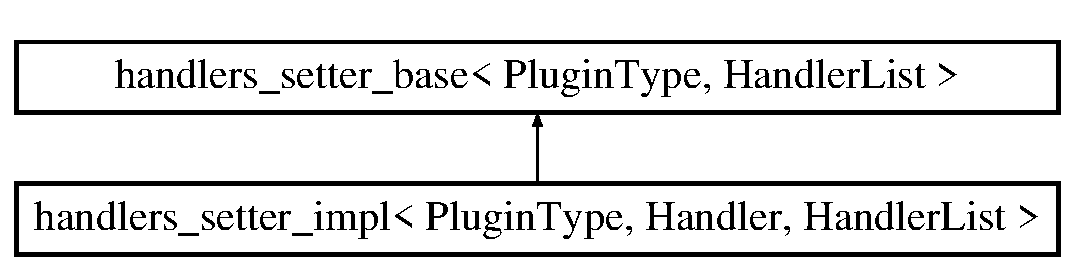
\includegraphics[height=2cm]{structhandlers__setter__base}
\end{center}
\end{figure}
\subsection*{Public Types}
\begin{CompactItemize}
\item 
\hypertarget{structhandlers__setter__base_50f6159e54d3b169f2f0ce5f80d865b4}{
typedef handlers\_\-setter$<$ PluginType, HandlerList $>$::type \textbf{next}}
\label{structhandlers__setter__base_50f6159e54d3b169f2f0ce5f80d865b4}

\end{CompactItemize}


\subsection{Detailed Description}
\subsubsection*{template$<$typename PluginType, typename HandlerList$>$ struct handlers\_\-setter\_\-base$<$ PluginType, HandlerList $>$}

\hyperlink{structhandlers__setter__base}{handlers\_\-setter\_\-base} will decide which our next setter will be 

The documentation for this struct was generated from the following file:\begin{CompactItemize}
\item 
include/lighttpd-cpp/handler\_\-helpers.hpp\end{CompactItemize}

\hypertarget{structhandlers__setter__end}{
\section{handlers\_\-setter\_\-end Struct Reference}
\label{structhandlers__setter__end}\index{handlers\_\-setter\_\-end@{handlers\_\-setter\_\-end}}
}
{\tt \#include $<$handler\_\-helpers.hpp$>$}

\subsection*{Static Public Member Functions}
\begin{CompactItemize}
\item 
\hypertarget{structhandlers__setter__end_6072b8c4d09f5d83388845fa228164ae}{
static void \textbf{set} (\hyperlink{structplugin}{plugin} \&p)}
\label{structhandlers__setter__end_6072b8c4d09f5d83388845fa228164ae}

\end{CompactItemize}


\subsection{Detailed Description}
When we reach \hyperlink{structhandlers__setter__end}{handlers\_\-setter\_\-end}, we are at the end of the HandlerList 

The documentation for this struct was generated from the following file:\begin{CompactItemize}
\item 
include/lighttpd-cpp/handler\_\-helpers.hpp\end{CompactItemize}

\hypertarget{structhandlers__setter__impl}{
\section{handlers\_\-setter\_\-impl$<$ PluginType, Handler, HandlerList $>$ Struct Template Reference}
\label{structhandlers__setter__impl}\index{handlers\_\-setter\_\-impl@{handlers\_\-setter\_\-impl}}
}
{\tt \#include $<$handler\_\-helpers.hpp$>$}

Inheritance diagram for handlers\_\-setter\_\-impl$<$ PluginType, Handler, HandlerList $>$::\begin{figure}[H]
\begin{center}
\leavevmode
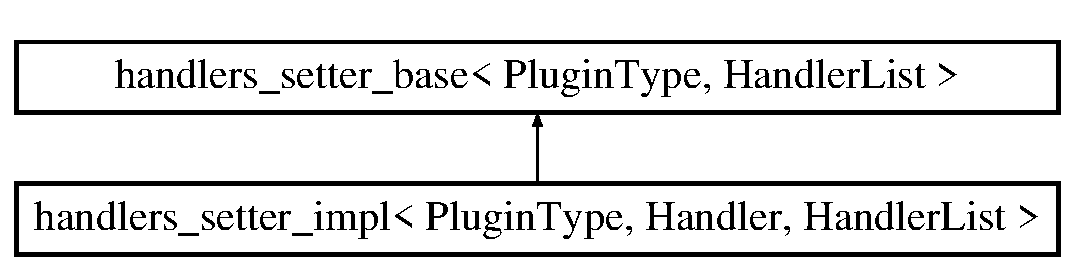
\includegraphics[height=2cm]{structhandlers__setter__impl}
\end{center}
\end{figure}


\subsection{Detailed Description}
\subsubsection*{template$<$typename PluginType, typename Handler, typename HandlerList$>$ struct handlers\_\-setter\_\-impl$<$ PluginType, Handler, HandlerList $>$}

Here we can partial specialize for Handler such that the right hook will be set. 

The documentation for this struct was generated from the following file:\begin{CompactItemize}
\item 
include/lighttpd-cpp/handler\_\-helpers.hpp\end{CompactItemize}

\hypertarget{structiosocket}{
\section{iosocket Struct Reference}
\label{structiosocket}\index{iosocket@{iosocket}}
}
{\tt \#include $<$iosocket.h$>$}

\subsection*{Public Attributes}
\begin{CompactItemize}
\item 
\hypertarget{structiosocket_c5dcd0d6bc41ffffa72a087555d012fc}{
int \textbf{fd}}
\label{structiosocket_c5dcd0d6bc41ffffa72a087555d012fc}

\item 
\hypertarget{structiosocket_ef7db9c046476d8fcbd24066daaa23bf}{
int \textbf{fde\_\-ndx}}
\label{structiosocket_ef7db9c046476d8fcbd24066daaa23bf}

\item 
iosocket\_\-t \hyperlink{structiosocket_4a478938dc364d5e9658b270039c5794}{type}
\end{CompactItemize}


\subsection{Detailed Description}
a non-blocking fd 

\subsection{Member Data Documentation}
\hypertarget{structiosocket_4a478938dc364d5e9658b270039c5794}{
\index{iosocket@{iosocket}!type@{type}}
\index{type@{type}!iosocket@{iosocket}}
\subsubsection[{type}]{\setlength{\rightskip}{0pt plus 5cm}iosocket\_\-t {\bf iosocket::type}}}
\label{structiosocket_4a478938dc364d5e9658b270039c5794}


sendfile on solaris doesn't work on pipes 

The documentation for this struct was generated from the following file:\begin{CompactItemize}
\item 
include/lighttpd/iosocket.h\end{CompactItemize}

\hypertarget{structplugin}{
\section{plugin Struct Reference}
\label{structplugin}\index{plugin@{plugin}}
}
{\tt \#include $<$plugin.h$>$}

\subsection*{Public Attributes}
\begin{CompactItemize}
\item 
\hypertarget{structplugin_a4b3d495a0ae1df759643b712d91068f}{
size\_\-t \textbf{version}}
\label{structplugin_a4b3d495a0ae1df759643b712d91068f}

\item 
\hypertarget{structplugin_235162d1645d005e4d8ea2cedc80a236}{
buffer $\ast$ \textbf{name}}
\label{structplugin_235162d1645d005e4d8ea2cedc80a236}

\item 
\hypertarget{structplugin_241bc6c5b4cb17a235b0947fac9d34d5}{
void $\ast$($\ast$ \textbf{init} )(server $\ast$srv)}
\label{structplugin_241bc6c5b4cb17a235b0947fac9d34d5}

\item 
\hypertarget{structplugin_04251883174cadf3e02ae1b1a388bdb7}{
handler\_\-t($\ast$ \textbf{set\_\-defaults} )(server $\ast$srv, void $\ast$p\_\-d)}
\label{structplugin_04251883174cadf3e02ae1b1a388bdb7}

\item 
\hypertarget{structplugin_c092882ffd286543515174a8bd3b70d2}{
handler\_\-t($\ast$ \textbf{cleanup} )(server $\ast$srv, void $\ast$p\_\-d)}
\label{structplugin_c092882ffd286543515174a8bd3b70d2}

\item 
\hypertarget{structplugin_6490af8e037a60d248395a8c68ee83f0}{
handler\_\-t($\ast$ \textbf{handle\_\-trigger} )(server $\ast$srv, void $\ast$p\_\-d)}
\label{structplugin_6490af8e037a60d248395a8c68ee83f0}

\item 
\hypertarget{structplugin_aa3aaf5324316058a36ab97ab7303a62}{
handler\_\-t($\ast$ \textbf{handle\_\-sighup} )(server $\ast$srv, void $\ast$p\_\-d)}
\label{structplugin_aa3aaf5324316058a36ab97ab7303a62}

\item 
\hypertarget{structplugin_e798106278e8cd7e7241b1f1ee9ac914}{
handler\_\-t($\ast$ \textbf{handle\_\-uri\_\-raw} )(server $\ast$srv, connection $\ast$con, void $\ast$p\_\-d)}
\label{structplugin_e798106278e8cd7e7241b1f1ee9ac914}

\item 
\hypertarget{structplugin_fc26fff5d1ec7666608fda729b6a9a74}{
handler\_\-t($\ast$ \textbf{handle\_\-uri\_\-clean} )(server $\ast$srv, connection $\ast$con, void $\ast$p\_\-d)}
\label{structplugin_fc26fff5d1ec7666608fda729b6a9a74}

\item 
\hypertarget{structplugin_c6e9dddb37aca959bd90651e949d5f4d}{
handler\_\-t($\ast$ \textbf{handle\_\-docroot} )(server $\ast$srv, connection $\ast$con, void $\ast$p\_\-d)}
\label{structplugin_c6e9dddb37aca959bd90651e949d5f4d}

\item 
\hypertarget{structplugin_e5818db20f5d464df84a4c8bf4354567}{
handler\_\-t($\ast$ \textbf{handle\_\-physical} )(server $\ast$srv, connection $\ast$con, void $\ast$p\_\-d)}
\label{structplugin_e5818db20f5d464df84a4c8bf4354567}

\item 
\hypertarget{structplugin_79a8993bebdb2ee0cfba7824468a694a}{
handler\_\-t($\ast$ \textbf{handle\_\-start\_\-backend} )(server $\ast$srv, connection $\ast$con, void $\ast$p\_\-d)}
\label{structplugin_79a8993bebdb2ee0cfba7824468a694a}

\item 
\hypertarget{structplugin_348b93d40df354c42d54ac743a6d2732}{
handler\_\-t($\ast$ \textbf{handle\_\-send\_\-request\_\-content} )(server $\ast$srv, connection $\ast$con, void $\ast$p\_\-d)}
\label{structplugin_348b93d40df354c42d54ac743a6d2732}

\item 
\hypertarget{structplugin_2c8efcd277395f7d1dbd484125cf5942}{
handler\_\-t($\ast$ \textbf{handle\_\-response\_\-header} )(server $\ast$srv, connection $\ast$con, void $\ast$p\_\-d)}
\label{structplugin_2c8efcd277395f7d1dbd484125cf5942}

\item 
\hypertarget{structplugin_2589836637d6c1520e21e08e97bc07f9}{
handler\_\-t($\ast$ \textbf{handle\_\-read\_\-response\_\-content} )(server $\ast$srv, connection $\ast$con, void $\ast$p\_\-d)}
\label{structplugin_2589836637d6c1520e21e08e97bc07f9}

\item 
\hypertarget{structplugin_4453042dcbc5c68c290f1451c580a46b}{
handler\_\-t($\ast$ \textbf{handle\_\-filter\_\-response\_\-content} )(server $\ast$srv, connection $\ast$con, void $\ast$p\_\-d)}
\label{structplugin_4453042dcbc5c68c290f1451c580a46b}

\item 
\hypertarget{structplugin_d464d2af155e15bb1ee88e91de6ff891}{
handler\_\-t($\ast$ \textbf{handle\_\-response\_\-done} )(server $\ast$srv, connection $\ast$con, void $\ast$p\_\-d)}
\label{structplugin_d464d2af155e15bb1ee88e91de6ff891}

\item 
\hypertarget{structplugin_5c3bbcff69dfdf5c591c0a420b38c055}{
handler\_\-t($\ast$ \textbf{connection\_\-reset} )(server $\ast$srv, connection $\ast$con, void $\ast$p\_\-d)}
\label{structplugin_5c3bbcff69dfdf5c591c0a420b38c055}

\item 
\hypertarget{structplugin_b59fbc651a4308ac4e89ed27d1d33a00}{
handler\_\-t($\ast$ \textbf{handle\_\-connection\_\-close} )(server $\ast$srv, connection $\ast$con, void $\ast$p\_\-d)}
\label{structplugin_b59fbc651a4308ac4e89ed27d1d33a00}

\item 
\hypertarget{structplugin_7d65846e47eeab07727ed3772d81e62b}{
handler\_\-t($\ast$ \textbf{handle\_\-joblist} )(server $\ast$srv, connection $\ast$con, void $\ast$p\_\-d)}
\label{structplugin_7d65846e47eeab07727ed3772d81e62b}

\item 
\hypertarget{structplugin_a5c0338878875f24bcaf3bb4e3f60bc6}{
void $\ast$ \textbf{data}}
\label{structplugin_a5c0338878875f24bcaf3bb4e3f60bc6}

\item 
\hypertarget{structplugin_b8a4a02c20d1fa7be51580e5c7584998}{
void $\ast$ \textbf{lib}}
\label{structplugin_b8a4a02c20d1fa7be51580e5c7584998}

\item 
\hypertarget{structplugin_bafa5fa5df2ab1a99454e7e56a5dbd61}{
array $\ast$ \textbf{required\_\-plugins}}
\label{structplugin_bafa5fa5df2ab1a99454e7e56a5dbd61}

\end{CompactItemize}


\subsection{Detailed Description}
we have 4 states on the connection:\begin{itemize}
\item read-header\item read-content\item write-header\item write-content \end{itemize}


The documentation for this struct was generated from the following file:\begin{CompactItemize}
\item 
include/lighttpd/plugin.h\end{CompactItemize}

\hypertarget{classPlugin}{
\section{Plugin$<$ MostDerived $>$ Class Template Reference}
\label{classPlugin}\index{Plugin@{Plugin}}
}
{\tt \#include $<$plugin.hpp$>$}

Inheritance diagram for Plugin$<$ MostDerived $>$::\begin{figure}[H]
\begin{center}
\leavevmode
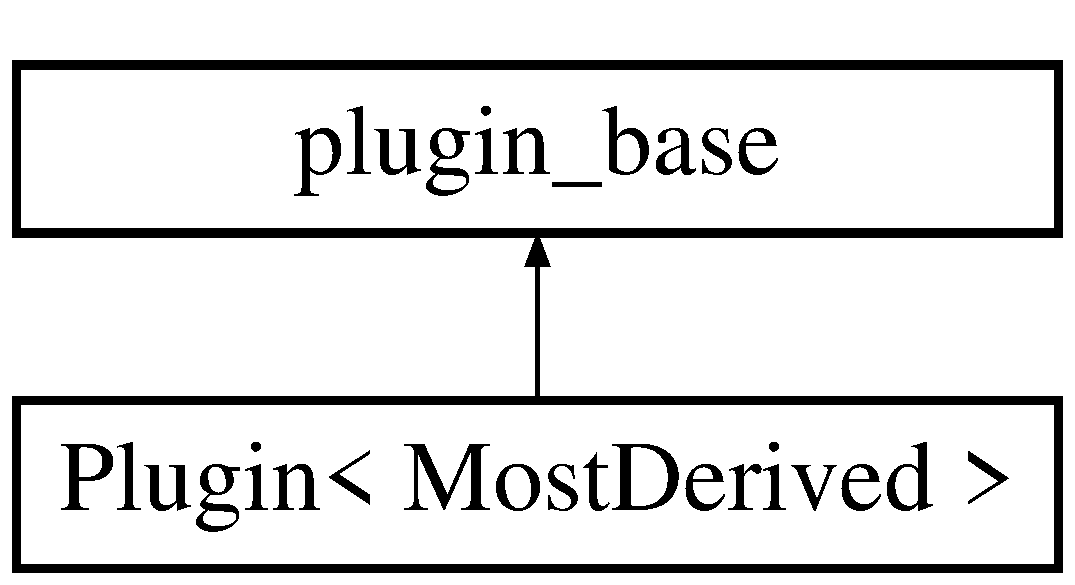
\includegraphics[height=2cm]{classPlugin}
\end{center}
\end{figure}
\subsection*{Static Public Member Functions}
\begin{CompactItemize}
\item 
\hypertarget{classPlugin_37ff1cb61a63833adee3cd4c0df42848}{
static int \textbf{create\_\-plugin} (\hyperlink{structplugin}{plugin} \&p)}
\label{classPlugin_37ff1cb61a63833adee3cd4c0df42848}

\end{CompactItemize}
\subsection*{Protected Member Functions}
\begin{CompactItemize}
\item 
\hypertarget{classPlugin_3e13aa67b9728e5accd83c41b9129b57}{
\textbf{Plugin} (const char $\ast$name, const std::size\_\-t version, \hyperlink{structplugin}{plugin} \&p)}
\label{classPlugin_3e13aa67b9728e5accd83c41b9129b57}

\end{CompactItemize}


\subsection{Detailed Description}
\subsubsection*{template$<$typename MostDerived$>$ class Plugin$<$ MostDerived $>$}

Abstract \hyperlink{structplugin}{plugin} base-class for plugins, non-constructable, hidden from C compilers. An alternative would be to have a \hyperlink{structplugin}{plugin} type derived from this for each handler type. 

The documentation for this class was generated from the following file:\begin{CompactItemize}
\item 
include/lighttpd-cpp/plugin.hpp\end{CompactItemize}

\hypertarget{classplugin__base}{
\section{plugin\_\-base Class Reference}
\label{classplugin__base}\index{plugin\_\-base@{plugin\_\-base}}
}
{\tt \#include $<$plugin.hpp$>$}

Inheritance diagram for plugin\_\-base::\begin{figure}[H]
\begin{center}
\leavevmode
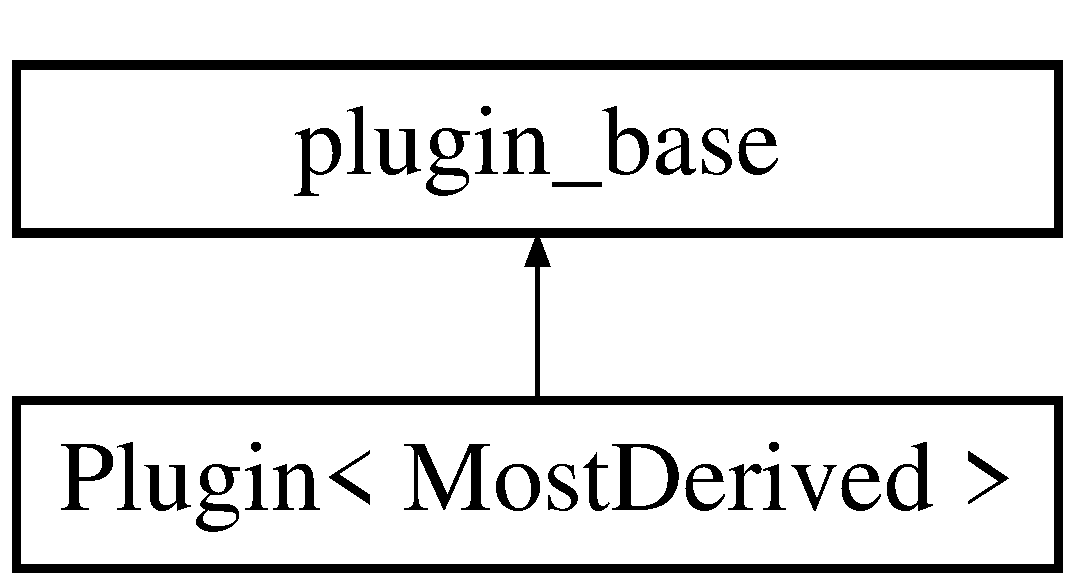
\includegraphics[height=2cm]{classplugin__base}
\end{center}
\end{figure}
\subsection*{Public Member Functions}
\begin{CompactItemize}
\item 
\hypertarget{classplugin__base_98a9f4ac48860934a8c1e96218e0cbf8}{
handler\_\-t \textbf{set\_\-defaults} ()}
\label{classplugin__base_98a9f4ac48860934a8c1e96218e0cbf8}

\item 
\hypertarget{classplugin__base_9e7d7fe3bfd0e4fac9d8cc4c88b19d06}{
void $\ast$ \textbf{initialize} (const server \&s)}
\label{classplugin__base_9e7d7fe3bfd0e4fac9d8cc4c88b19d06}

\end{CompactItemize}
\subsection*{Static Public Member Functions}
\begin{CompactItemize}
\item 
\hypertarget{classplugin__base_1fa7efbeb3925de31e1e59186658c1c0}{
static handler\_\-t \textbf{set\_\-defaults\_\-wrapper} (server $\ast$s, void $\ast$p\_\-d)}
\label{classplugin__base_1fa7efbeb3925de31e1e59186658c1c0}

\item 
\hypertarget{classplugin__base_3f93f1b89e4494a4c389115c8ef005b2}{
static void $\ast$ \textbf{initialize\_\-wrapper} (server $\ast$s, void $\ast$p\_\-d)}
\label{classplugin__base_3f93f1b89e4494a4c389115c8ef005b2}

\end{CompactItemize}
\subsection*{Protected Member Functions}
\begin{CompactItemize}
\item 
\hypertarget{classplugin__base_7ce2c669c0efe22575ca69b3becdc237}{
\textbf{plugin\_\-base} (const char $\ast$name, const std::size\_\-t version, \hyperlink{structplugin}{plugin} \&p)}
\label{classplugin__base_7ce2c669c0efe22575ca69b3becdc237}

\end{CompactItemize}
\subsection*{Protected Attributes}
\begin{CompactItemize}
\item 
\hypertarget{classplugin__base_6e26cf6e1b55bc4a0c3d80cc57553e67}{
\hyperlink{structplugin}{plugin} \& \textbf{p}}
\label{classplugin__base_6e26cf6e1b55bc4a0c3d80cc57553e67}

\item 
\hypertarget{classplugin__base_e21602a179186848d2683d5203d811fe}{
const server $\ast$ \textbf{srv}}
\label{classplugin__base_e21602a179186848d2683d5203d811fe}

\end{CompactItemize}


\subsection{Detailed Description}
Base class for deriving C++ plugins from. Possibly useful if you like this sort of thing. Otherwise just make use you extern the appropriate functions (i.e. the \hyperlink{structplugin}{plugin} init function) to have C symbols. Abstract base class for C++ lighty plugins. Not sure if its worth it yet, lets see how useful it is. Really there shouldn't be any significant performance hit with these wrappers, only a small increase in memory usage per \hyperlink{structplugin}{plugin} (irrelivant). Other hit due to function calling convensions for which I do not know the details.

Things that need encapsulating:

\hyperlink{classPlugin}{Plugin} house keeping:\begin{itemize}
\item set which part of the request flow we handle. i.e. \_\-plugin\_\-init\item populate \hyperlink{structplugin}{plugin} config. i.e. set\_\-defaults\item clean up allocated memory we used. i.e. cleanup\end{itemize}


The request flow:\begin{itemize}
\item HTTP request recieved, i.e. protocol, method, uri\_\-raw, headers (see http\_\-req.h)\item \char`\"{}Clean\char`\"{} uri\_\-raw -$>$ uri\_\-clean i.e. mod\_\-rewrite\item Map the clean request to an appropriate docroot.\item Get the physical path to the requested file.\item Do untold horrors to the requested file.\begin{itemize}
\item More things here.\end{itemize}
\item Send a response back maybe.\end{itemize}


Lighty allows plugins to hook in to multiple points of this flow, i.e. one type of \hyperlink{structplugin}{plugin}, but their effects at certain levels may be NULL. Serves as an easy method of sharing data between points of flow. Perhaps theres something in trying to abstract this shared data out, and removing this hardcoded sharing within a \hyperlink{structplugin}{plugin}. Don't know, just a gut feeling. Absolute base for plugins. 

The documentation for this class was generated from the following file:\begin{CompactItemize}
\item 
include/lighttpd-cpp/plugin.hpp\end{CompactItemize}

\hypertarget{structplugin__config}{
\section{plugin\_\-config Struct Reference}
\label{structplugin__config}\index{plugin\_\-config@{plugin\_\-config}}
}
\subsection*{Public Attributes}
\begin{CompactItemize}
\item 
\hypertarget{structplugin__config_f503027bbb7fb2345bf6ac966a3f94d4}{
array $\ast$ \textbf{access\_\-deny}}
\label{structplugin__config_f503027bbb7fb2345bf6ac966a3f94d4}

\item 
\hypertarget{structplugin__config_d64be108cd5d2f0cbbb1bbf6987a4261}{
unsigned short \textbf{deny\_\-all}}
\label{structplugin__config_d64be108cd5d2f0cbbb1bbf6987a4261}

\item 
\hypertarget{structplugin__config_9f49dacad1547afc5c4f342e2785b890}{
buffer $\ast$ \textbf{access\_\-logfile}}
\label{structplugin__config_9f49dacad1547afc5c4f342e2785b890}

\item 
\hypertarget{structplugin__config_f1cea69ff3a5d21625609be6668fa138}{
buffer $\ast$ \textbf{format}}
\label{structplugin__config_f1cea69ff3a5d21625609be6668fa138}

\item 
\hypertarget{structplugin__config_0550af5388be0c53c8e7d608ab13223a}{
unsigned short \textbf{use\_\-syslog}}
\label{structplugin__config_0550af5388be0c53c8e7d608ab13223a}

\item 
\hypertarget{structplugin__config_c2cfe959ecfdb9e94aa13fb163c58e85}{
int \textbf{log\_\-access\_\-fd}}
\label{structplugin__config_c2cfe959ecfdb9e94aa13fb163c58e85}

\item 
\hypertarget{structplugin__config_e3bcf96bb33e24cd8757fc9a4c90825b}{
time\_\-t \textbf{last\_\-generated\_\-accesslog\_\-ts}}
\label{structplugin__config_e3bcf96bb33e24cd8757fc9a4c90825b}

\item 
\hypertarget{structplugin__config_d23655083ebea6a8d9f9a21c9827c7e7}{
time\_\-t $\ast$ \textbf{last\_\-generated\_\-accesslog\_\-ts\_\-ptr}}
\label{structplugin__config_d23655083ebea6a8d9f9a21c9827c7e7}

\item 
\hypertarget{structplugin__config_c96f3c49710be2e36f04124164f3e68e}{
buffer $\ast$ \textbf{access\_\-logbuffer}}
\label{structplugin__config_c96f3c49710be2e36f04124164f3e68e}

\item 
\hypertarget{structplugin__config_4fbaad72d7ba8e7f74f52ab59f20a9e3}{
buffer $\ast$ \textbf{ts\_\-accesslog\_\-str}}
\label{structplugin__config_4fbaad72d7ba8e7f74f52ab59f20a9e3}

\item 
\hypertarget{structplugin__config_987497c9c45b892fd54523000650dd8a}{
format\_\-fields $\ast$ \textbf{parsed\_\-format}}
\label{structplugin__config_987497c9c45b892fd54523000650dd8a}

\item 
\hypertarget{structplugin__config_54b001d895399c170c3911957611c797}{
array $\ast$ \textbf{alias}}
\label{structplugin__config_54b001d895399c170c3911957611c797}

\item 
\hypertarget{structplugin__config_1e820d2000c648348113f8eab880541e}{
array $\ast$ \textbf{cgi}}
\label{structplugin__config_1e820d2000c648348113f8eab880541e}

\item 
\hypertarget{structplugin__config_1160174309e0ce58b2a7c89b0abcb553}{
unsigned short \textbf{execute\_\-all}}
\label{structplugin__config_1160174309e0ce58b2a7c89b0abcb553}

\item 
\hypertarget{structplugin__config_de3cfcb6c674c770a6e7c5c352476383}{
unsigned short \textbf{execute\_\-x\_\-only}}
\label{structplugin__config_de3cfcb6c674c770a6e7c5c352476383}

\item 
\hypertarget{structplugin__config_55f1d6f5cbe3583dcfe67709f36b4612}{
unsigned short \textbf{encoding}}
\label{structplugin__config_55f1d6f5cbe3583dcfe67709f36b4612}

\item 
\hypertarget{structplugin__config_8d6b7c8c9974668b8a6cf70e7b7a33ac}{
unsigned short \textbf{debug}}
\label{structplugin__config_8d6b7c8c9974668b8a6cf70e7b7a33ac}

\item 
\hypertarget{structplugin__config_0b46108e6b03529131edf5267fb2901e}{
buffer $\ast$ \textbf{compress\_\-cache\_\-dir}}
\label{structplugin__config_0b46108e6b03529131edf5267fb2901e}

\item 
\hypertarget{structplugin__config_7932fcac5458d93837e7e6e3afffa6a4}{
array $\ast$ \textbf{compress}}
\label{structplugin__config_7932fcac5458d93837e7e6e3afffa6a4}

\item 
\hypertarget{structplugin__config_f5ebee1c843bd5f9c79bcda3abe37872}{
off\_\-t \textbf{compress\_\-max\_\-filesize}}
\label{structplugin__config_f5ebee1c843bd5f9c79bcda3abe37872}

\item 
int \hyperlink{structplugin__config_7a925bb5a8cf2be24c6f4db3cb3f9006}{allowed\_\-encodings}
\item 
\hypertarget{structplugin__config_d98acc4cd9c78b8fbdbf86b7329684f7}{
unsigned short \textbf{enabled}}
\label{structplugin__config_d98acc4cd9c78b8fbdbf86b7329684f7}

\item 
\hypertarget{structplugin__config_f474def361a549cc0b8e719d4af2fc68}{
unsigned short \textbf{sync\_\-flush}}
\label{structplugin__config_f474def361a549cc0b8e719d4af2fc68}

\item 
\hypertarget{structplugin__config_746003a87ec7a397f6a12d4d677de0fe}{
unsigned short \textbf{output\_\-buffer\_\-size}}
\label{structplugin__config_746003a87ec7a397f6a12d4d677de0fe}

\item 
\hypertarget{structplugin__config_0b8e331453deca106e79afb2e96e75a1}{
unsigned short \textbf{min\_\-compress\_\-size}}
\label{structplugin__config_0b8e331453deca106e79afb2e96e75a1}

\item 
\hypertarget{structplugin__config_e9d80653853b7571ce08b5c358bf8853}{
unsigned short \textbf{work\_\-block\_\-size}}
\label{structplugin__config_e9d80653853b7571ce08b5c358bf8853}

\item 
\hypertarget{structplugin__config_a3de5b8c5880b6f752e679610918610e}{
short \textbf{mem\_\-level}}
\label{structplugin__config_a3de5b8c5880b6f752e679610918610e}

\item 
\hypertarget{structplugin__config_2600cca34919dfb16950767fa9a2a604}{
short \textbf{compression\_\-level}}
\label{structplugin__config_2600cca34919dfb16950767fa9a2a604}

\item 
\hypertarget{structplugin__config_3f41b3f585474524badfcf53b5c6c7bc}{
short \textbf{window\_\-size}}
\label{structplugin__config_3f41b3f585474524badfcf53b5c6c7bc}

\item 
\hypertarget{structplugin__config_57d3457480703ae7f40e0ada85cf25ef}{
array $\ast$ \textbf{mimetypes}}
\label{structplugin__config_57d3457480703ae7f40e0ada85cf25ef}

\item 
\hypertarget{structplugin__config_340eeb9fec7e2eedaf7d09372a49aad6}{
unsigned short \textbf{dir\_\-listing}}
\label{structplugin__config_340eeb9fec7e2eedaf7d09372a49aad6}

\item 
\hypertarget{structplugin__config_e22fc24e78563e179fc8f5c5d66908d8}{
unsigned short \textbf{hide\_\-dot\_\-files}}
\label{structplugin__config_e22fc24e78563e179fc8f5c5d66908d8}

\item 
\hypertarget{structplugin__config_b883ea99311fd959b5c050d292cfec29}{
unsigned short \textbf{show\_\-readme}}
\label{structplugin__config_b883ea99311fd959b5c050d292cfec29}

\item 
\hypertarget{structplugin__config_7e495d4e5ef0b6cbe7f89c8f0051344a}{
unsigned short \textbf{hide\_\-readme\_\-file}}
\label{structplugin__config_7e495d4e5ef0b6cbe7f89c8f0051344a}

\item 
\hypertarget{structplugin__config_10a150543bb6c551136ee8ef14b3fd3b}{
unsigned short \textbf{show\_\-header}}
\label{structplugin__config_10a150543bb6c551136ee8ef14b3fd3b}

\item 
\hypertarget{structplugin__config_20efae724b908d84708092c243bdbfec}{
unsigned short \textbf{hide\_\-header\_\-file}}
\label{structplugin__config_20efae724b908d84708092c243bdbfec}

\item 
\hypertarget{structplugin__config_8d5a7a71f3091b091a37b08f5481b16f}{
excludes\_\-buffer $\ast$ \textbf{excludes}}
\label{structplugin__config_8d5a7a71f3091b091a37b08f5481b16f}

\item 
\hypertarget{structplugin__config_0de3019ee9404f690458f15c08d8f790}{
buffer $\ast$ \textbf{external\_\-css}}
\label{structplugin__config_0de3019ee9404f690458f15c08d8f790}

\item 
\hypertarget{structplugin__config_0f9e219aa12e75027ecec74bfccebdb5}{
buffer $\ast$ \textbf{encoding}}
\label{structplugin__config_0f9e219aa12e75027ecec74bfccebdb5}

\item 
\hypertarget{structplugin__config_6051c6eccfe87465909ddc25490d5311}{
buffer $\ast$ \textbf{set\_\-footer}}
\label{structplugin__config_6051c6eccfe87465909ddc25490d5311}

\item 
\hypertarget{structplugin__config_e594c7b02113f968a3f54ed5eac7d450}{
unsigned short \textbf{max\_\-conns}}
\label{structplugin__config_e594c7b02113f968a3f54ed5eac7d450}

\item 
\hypertarget{structplugin__config_ec0e007f1d17359a43373ec7103255a5}{
buffer $\ast$ \textbf{path\_\-pieces\_\-raw}}
\label{structplugin__config_ec0e007f1d17359a43373ec7103255a5}

\item 
\hypertarget{structplugin__config_99f095cf4d13dc80a2f684ef20b4195d}{
size\_\-t \textbf{len}}
\label{structplugin__config_99f095cf4d13dc80a2f684ef20b4195d}

\item 
\hypertarget{structplugin__config_d893918703f5468a3237aed674073194}{
buffer $\ast$$\ast$ \textbf{path\_\-pieces}}
\label{structplugin__config_d893918703f5468a3237aed674073194}

\item 
\hypertarget{structplugin__config_22279a8ba759ef86b05dfe068e312f02}{
array $\ast$ \textbf{expire\_\-url}}
\label{structplugin__config_22279a8ba759ef86b05dfe068e312f02}

\item 
\hypertarget{structplugin__config_07d0f56591824bb320237d6e4fc5c503}{
array $\ast$ \textbf{extensions}}
\label{structplugin__config_07d0f56591824bb320237d6e4fc5c503}

\item 
\hypertarget{structplugin__config_d3deb44ffab7392c14dcf06c9336d094}{
array $\ast$ \textbf{indexfiles}}
\label{structplugin__config_d3deb44ffab7392c14dcf06c9336d094}

\item 
\hypertarget{structplugin__config_12533b6e590e258a9676ab083e191040}{
proxy\_\-backends $\ast$ \textbf{backends}}
\label{structplugin__config_12533b6e590e258a9676ab083e191040}

\item 
\hypertarget{structplugin__config_bdc4055b945583f51b38311781911562}{
\hyperlink{structproxy__backlog}{proxy\_\-backlog} $\ast$ \textbf{backlog}}
\label{structplugin__config_bdc4055b945583f51b38311781911562}

\item 
\hypertarget{structplugin__config_993488a5c032a5a2f2a1e63b90dff13b}{
data\_\-integer $\ast$ \textbf{backlog\_\-size}}
\label{structplugin__config_993488a5c032a5a2f2a1e63b90dff13b}

\item 
\hypertarget{structplugin__config_a7f8b417d0e9faeb9df73de6e26a9508}{
proxy\_\-rewrites $\ast$ \textbf{request\_\-rewrites}}
\label{structplugin__config_a7f8b417d0e9faeb9df73de6e26a9508}

\item 
\hypertarget{structplugin__config_333223212c27619c6e103ce23c90024e}{
proxy\_\-rewrites $\ast$ \textbf{response\_\-rewrites}}
\label{structplugin__config_333223212c27619c6e103ce23c90024e}

\item 
\hypertarget{structplugin__config_276fbfe9afa48c542130c1e9e959edc2}{
unsigned short \textbf{allow\_\-x\_\-sendfile}}
\label{structplugin__config_276fbfe9afa48c542130c1e9e959edc2}

\item 
\hypertarget{structplugin__config_b9436c96cfd198d89cc003ecd8847780}{
unsigned short \textbf{allow\_\-x\_\-rewrite}}
\label{structplugin__config_b9436c96cfd198d89cc003ecd8847780}

\item 
\hypertarget{structplugin__config_788cd252dad57bbbc61c2b02d7231674}{
unsigned short \textbf{max\_\-pool\_\-size}}
\label{structplugin__config_788cd252dad57bbbc61c2b02d7231674}

\item 
\hypertarget{structplugin__config_f534be9f6bf0ff2b139b653206ee13df}{
unsigned short \textbf{check\_\-local}}
\label{structplugin__config_f534be9f6bf0ff2b139b653206ee13df}

\item 
\hypertarget{structplugin__config_ee8fbf3b1e55457419401116281a53bf}{
unsigned short \textbf{split\_\-hostnames}}
\label{structplugin__config_ee8fbf3b1e55457419401116281a53bf}

\item 
\hypertarget{structplugin__config_8e959bc85e9f8c7b4db3d10dba6708e0}{
unsigned short \textbf{max\_\-keep\_\-alive\_\-requests}}
\label{structplugin__config_8e959bc85e9f8c7b4db3d10dba6708e0}

\item 
\hypertarget{structplugin__config_c4f0cd0d905bca88acb00016507fe5d1}{
proxy\_\-balance\_\-t \textbf{balancer}}
\label{structplugin__config_c4f0cd0d905bca88acb00016507fe5d1}

\item 
\hypertarget{structplugin__config_4440ae76d0d9615f789f70f1062ed989}{
struct proxy\_\-protocol $\ast$ \textbf{protocol}}
\label{structplugin__config_4440ae76d0d9615f789f70f1062ed989}

\item 
\hypertarget{structplugin__config_02dd868b2860bc543c281ce27a347b77}{
pcre\_\-keyvalue\_\-buffer $\ast$ \textbf{redirect}}
\label{structplugin__config_02dd868b2860bc543c281ce27a347b77}

\item 
\hypertarget{structplugin__config_01a6b45dfa3166e09e9034670616c4a4}{
data\_\-config $\ast$ \textbf{context}}
\label{structplugin__config_01a6b45dfa3166e09e9034670616c4a4}

\item 
\hypertarget{structplugin__config_a64d0c0d3295ca55475831bdba40bec9}{
unsigned short \textbf{redirect\_\-code}}
\label{structplugin__config_a64d0c0d3295ca55475831bdba40bec9}

\item 
\hypertarget{structplugin__config_3fdacbf86b1c09e4238b20ffb43cf81f}{
pcre\_\-keyvalue\_\-buffer $\ast$ \textbf{rewrite}}
\label{structplugin__config_3fdacbf86b1c09e4238b20ffb43cf81f}

\item 
\hypertarget{structplugin__config_2908a2f50239c6098533b5be9b05e8cd}{
buffer $\ast$ \textbf{once}}
\label{structplugin__config_2908a2f50239c6098533b5be9b05e8cd}

\item 
\hypertarget{structplugin__config_c7180097e35afa33527e0559de42634f}{
buffer $\ast$ \textbf{path\_\-rrdtool\_\-bin}}
\label{structplugin__config_c7180097e35afa33527e0559de42634f}

\item 
\hypertarget{structplugin__config_2c786a61295bfbae1e70c44aa2d25b5d}{
buffer $\ast$ \textbf{path\_\-rrd}}
\label{structplugin__config_2c786a61295bfbae1e70c44aa2d25b5d}

\item 
\hypertarget{structplugin__config_7254db6479d2b2ca596b0615cfbf1e52}{
double \textbf{requests}}
\label{structplugin__config_7254db6479d2b2ca596b0615cfbf1e52}

\item 
\hypertarget{structplugin__config_419904fb4dba3b8b2497c89c8550ece7}{
double $\ast$ \textbf{requests\_\-ptr}}
\label{structplugin__config_419904fb4dba3b8b2497c89c8550ece7}

\item 
\hypertarget{structplugin__config_7918a8c2b4842e7783e02297c2f614ee}{
double \textbf{bytes\_\-written}}
\label{structplugin__config_7918a8c2b4842e7783e02297c2f614ee}

\item 
\hypertarget{structplugin__config_1b61b44961e306b46d98c354d141ccec}{
double $\ast$ \textbf{bytes\_\-written\_\-ptr}}
\label{structplugin__config_1b61b44961e306b46d98c354d141ccec}

\item 
\hypertarget{structplugin__config_23c664d4a7e04e73cadd7da496f81fab}{
double \textbf{bytes\_\-read}}
\label{structplugin__config_23c664d4a7e04e73cadd7da496f81fab}

\item 
\hypertarget{structplugin__config_b4bd126e1de23cb09e70c54454281b52}{
double $\ast$ \textbf{bytes\_\-read\_\-ptr}}
\label{structplugin__config_b4bd126e1de23cb09e70c54454281b52}

\item 
\hypertarget{structplugin__config_8ba5a42020918c4727aacac451f3e720}{
buffer $\ast$ \textbf{doc\_\-root}}
\label{structplugin__config_8ba5a42020918c4727aacac451f3e720}

\item 
\hypertarget{structplugin__config_5b94a0762750cc54bb38e15eb1804a1e}{
buffer $\ast$ \textbf{secret}}
\label{structplugin__config_5b94a0762750cc54bb38e15eb1804a1e}

\item 
\hypertarget{structplugin__config_ef05c144457960745a6747518cc5f0d1}{
buffer $\ast$ \textbf{uri\_\-prefix}}
\label{structplugin__config_ef05c144457960745a6747518cc5f0d1}

\item 
\hypertarget{structplugin__config_0075ba20f2b1935b3731eb583a5b0052}{
unsigned int \textbf{timeout}}
\label{structplugin__config_0075ba20f2b1935b3731eb583a5b0052}

\item 
\hypertarget{structplugin__config_e02d4e475dc2263c8b30e000712ba940}{
array $\ast$ \textbf{request\_\-header}}
\label{structplugin__config_e02d4e475dc2263c8b30e000712ba940}

\item 
\hypertarget{structplugin__config_fc9d60926d1c47c62278bec1ded34470}{
array $\ast$ \textbf{response\_\-header}}
\label{structplugin__config_fc9d60926d1c47c62278bec1ded34470}

\item 
\hypertarget{structplugin__config_ed7cc4d4346ffca4a1a6f0a77865ceef}{
array $\ast$ \textbf{environment}}
\label{structplugin__config_ed7cc4d4346ffca4a1a6f0a77865ceef}

\item 
\hypertarget{structplugin__config_5d8982f6bebb4ce309f7eb6837e6dd3b}{
buffer $\ast$ \textbf{server\_\-root}}
\label{structplugin__config_5d8982f6bebb4ce309f7eb6837e6dd3b}

\item 
\hypertarget{structplugin__config_f5f66a923a5857c6c7ede0bd5be2f624}{
buffer $\ast$ \textbf{default\_\-host}}
\label{structplugin__config_f5f66a923a5857c6c7ede0bd5be2f624}

\item 
\hypertarget{structplugin__config_1e881c816cbb849873b45a53c6937f4c}{
buffer $\ast$ \textbf{document\_\-root}}
\label{structplugin__config_1e881c816cbb849873b45a53c6937f4c}

\item 
\hypertarget{structplugin__config_ced1c921d3daf96fb443821f19420a98}{
buffer $\ast$ \textbf{docroot\_\-cache\_\-key}}
\label{structplugin__config_ced1c921d3daf96fb443821f19420a98}

\item 
\hypertarget{structplugin__config_200b47985e662bd13047a2118952e62e}{
buffer $\ast$ \textbf{docroot\_\-cache\_\-value}}
\label{structplugin__config_200b47985e662bd13047a2118952e62e}

\item 
\hypertarget{structplugin__config_76c0e6a6dc25c344441e75feeb7b673f}{
buffer $\ast$ \textbf{docroot\_\-cache\_\-servername}}
\label{structplugin__config_76c0e6a6dc25c344441e75feeb7b673f}

\item 
\hypertarget{structplugin__config_7a3c933dffd1f29673281c093373acf6}{
array $\ast$ \textbf{match}}
\label{structplugin__config_7a3c933dffd1f29673281c093373acf6}

\item 
\hypertarget{structplugin__config_3a055b2a593ee988adf29f98b3524475}{
array $\ast$ \textbf{ssi\_\-extension}}
\label{structplugin__config_3a055b2a593ee988adf29f98b3524475}

\item 
\hypertarget{structplugin__config_8c7734d100c6746915cdce4b36696f9d}{
buffer $\ast$ \textbf{content\_\-type}}
\label{structplugin__config_8c7734d100c6746915cdce4b36696f9d}

\item 
\hypertarget{structplugin__config_2cf350729e68bc790cdf2ecfa10107b5}{
array $\ast$ \textbf{exclude\_\-ext}}
\label{structplugin__config_2cf350729e68bc790cdf2ecfa10107b5}

\item 
\hypertarget{structplugin__config_72d94ba8d09b9d0c19d225f804783ea0}{
buffer $\ast$ \textbf{config\_\-url}}
\label{structplugin__config_72d94ba8d09b9d0c19d225f804783ea0}

\item 
\hypertarget{structplugin__config_44b94ae3dac658262e9900c15f20c185}{
buffer $\ast$ \textbf{status\_\-url}}
\label{structplugin__config_44b94ae3dac658262e9900c15f20c185}

\item 
\hypertarget{structplugin__config_3d8f2557d9fdee9bec842e2cdb091130}{
buffer $\ast$ \textbf{statistics\_\-url}}
\label{structplugin__config_3d8f2557d9fdee9bec842e2cdb091130}

\item 
\hypertarget{structplugin__config_23038956d73aa3c2e2d167a7623f7466}{
int \textbf{sort}}
\label{structplugin__config_23038956d73aa3c2e2d167a7623f7466}

\item 
\hypertarget{structplugin__config_d9b213b7075614a9e16ea2fe01616417}{
buffer $\ast$ \textbf{db\_\-filename}}
\label{structplugin__config_d9b213b7075614a9e16ea2fe01616417}

\item 
\hypertarget{structplugin__config_d6e253381a98c1de44924079f56aef61}{
buffer $\ast$ \textbf{trigger\_\-url}}
\label{structplugin__config_d6e253381a98c1de44924079f56aef61}

\item 
\hypertarget{structplugin__config_0acdf0db3f564be268cdaa3b7efd0319}{
buffer $\ast$ \textbf{download\_\-url}}
\label{structplugin__config_0acdf0db3f564be268cdaa3b7efd0319}

\item 
\hypertarget{structplugin__config_644e3ac75c5cc8c851157b93f392e7cf}{
buffer $\ast$ \textbf{deny\_\-url}}
\label{structplugin__config_644e3ac75c5cc8c851157b93f392e7cf}

\item 
\hypertarget{structplugin__config_898db70a1bdc806d1a8a7cd4eaa75b64}{
array $\ast$ \textbf{mc\_\-hosts}}
\label{structplugin__config_898db70a1bdc806d1a8a7cd4eaa75b64}

\item 
\hypertarget{structplugin__config_b72b78eb836631c219313915c892e15c}{
buffer $\ast$ \textbf{mc\_\-namespace}}
\label{structplugin__config_b72b78eb836631c219313915c892e15c}

\item 
\hypertarget{structplugin__config_c3d0a604deae5fe7540830d91f6196f6}{
unsigned short \textbf{trigger\_\-timeout}}
\label{structplugin__config_c3d0a604deae5fe7540830d91f6196f6}

\item 
\hypertarget{structplugin__config_6260afa88f6d802feb2ccb3b7c729c9c}{
buffer $\ast$ \textbf{progress\_\-url}}
\label{structplugin__config_6260afa88f6d802feb2ccb3b7c729c9c}

\item 
\hypertarget{structplugin__config_f0c48929377cdcd052b96b60b158761f}{
unsigned short \textbf{remove\_\-timeout}}
\label{structplugin__config_f0c48929377cdcd052b96b60b158761f}

\item 
\hypertarget{structplugin__config_3ca541f13e7d19d371ecd4af89626039}{
array $\ast$ \textbf{exclude\_\-user}}
\label{structplugin__config_3ca541f13e7d19d371ecd4af89626039}

\item 
\hypertarget{structplugin__config_2f69bbbd86f6e71a68d83ea7584f5992}{
array $\ast$ \textbf{include\_\-user}}
\label{structplugin__config_2f69bbbd86f6e71a68d83ea7584f5992}

\item 
\hypertarget{structplugin__config_17b954d56b5f4454890fdad79f59294c}{
buffer $\ast$ \textbf{path}}
\label{structplugin__config_17b954d56b5f4454890fdad79f59294c}

\item 
\hypertarget{structplugin__config_cb95a158e6542864ded7fb961bdf4414}{
buffer $\ast$ \textbf{basepath}}
\label{structplugin__config_cb95a158e6542864ded7fb961bdf4414}

\item 
\hypertarget{structplugin__config_f2ebccceca2472128a4b4b1020061623}{
unsigned short \textbf{letterhomes}}
\label{structplugin__config_f2ebccceca2472128a4b4b1020061623}

\item 
\hypertarget{structplugin__config_32aab911a89b50b49652cfc7adcebb3c}{
buffer $\ast$ \textbf{cookie\_\-name}}
\label{structplugin__config_32aab911a89b50b49652cfc7adcebb3c}

\item 
\hypertarget{structplugin__config_393dbba4fefb1846530631039ac161da}{
buffer $\ast$ \textbf{cookie\_\-domain}}
\label{structplugin__config_393dbba4fefb1846530631039ac161da}

\item 
\hypertarget{structplugin__config_9f2851682f1841093eaf9c81c36c8eb9}{
unsigned short \textbf{cookie\_\-max\_\-age}}
\label{structplugin__config_9f2851682f1841093eaf9c81c36c8eb9}

\item 
\hypertarget{structplugin__config_e310e81d2c5196b21c0b47ef25dfd8c0}{
unsigned short \textbf{is\_\-readonly}}
\label{structplugin__config_e310e81d2c5196b21c0b47ef25dfd8c0}

\item 
\hypertarget{structplugin__config_d23b6f47f9027b70aafea3545f0bca07}{
unsigned short \textbf{log\_\-xml}}
\label{structplugin__config_d23b6f47f9027b70aafea3545f0bca07}

\item 
\hypertarget{structplugin__config_eb366b3184e29302be12a34ddfe85a2b}{
buffer $\ast$ \textbf{sqlite\_\-db\_\-name}}
\label{structplugin__config_eb366b3184e29302be12a34ddfe85a2b}

\end{CompactItemize}


\subsection{Detailed Description}
This \hyperlink{structplugin}{plugin} adds HTTP/1.1 chunked encoding support as a filter module.

mod\_\-evasive

we indent to implement all features the mod\_\-evasive from apache has

\begin{itemize}
\item limit of connections per IP\item provide a list of block-listed ip/networks (no access)\item provide a white-list of ips/network which is not affected by the limit (hmm, conditionals might be enough)\item provide a bandwidth limiter per IP\end{itemize}


started by:\begin{itemize}
\item \href{mailto:w1zzard@techpowerup.com}{\tt w1zzard@techpowerup.com}\end{itemize}


this is a expire module for a lighttpd

set 'Expires:' HTTP Headers on demand

this is a skeleton for a lighttpd \hyperlink{structplugin}{plugin}

just replaces every occurance of 'skeleton' by your \hyperlink{structplugin}{plugin} name

e.g. in vim:

:s/skeleton/myhandler/

this is a staticfile for a lighttpd \hyperlink{structplugin}{plugin}

this is a trigger\_\-b4\_\-dl for a lighttpd \hyperlink{structplugin}{plugin} 

\subsection{Member Data Documentation}
\hypertarget{structplugin__config_7a925bb5a8cf2be24c6f4db3cb3f9006}{
\index{plugin\_\-config@{plugin\_\-config}!allowed\_\-encodings@{allowed\_\-encodings}}
\index{allowed\_\-encodings@{allowed\_\-encodings}!plugin_config@{plugin\_\-config}}
\subsubsection[{allowed\_\-encodings}]{\setlength{\rightskip}{0pt plus 5cm}int {\bf plugin\_\-config::allowed\_\-encodings}}}
\label{structplugin__config_7a925bb5a8cf2be24c6f4db3cb3f9006}


max filesize in kb 

The documentation for this struct was generated from the following files:\begin{CompactItemize}
\item 
include/lighttpd/mod\_\-access.c\item 
include/lighttpd/mod\_\-accesslog.c\item 
include/lighttpd/mod\_\-alias.c\item 
include/lighttpd/mod\_\-cgi.c\item 
include/lighttpd/mod\_\-chunked.c\item 
include/lighttpd/mod\_\-compress.c\item 
include/lighttpd/mod\_\-deflate.c\item 
include/lighttpd/mod\_\-dirlisting.c\item 
include/lighttpd/mod\_\-evasive.c\item 
include/lighttpd/mod\_\-evhost.c\item 
include/lighttpd/mod\_\-expire.c\item 
include/lighttpd/mod\_\-flv\_\-streaming.c\item 
include/lighttpd/mod\_\-indexfile.c\item 
include/lighttpd/mod\_\-proxy\_\-core.h\item 
include/lighttpd/mod\_\-redirect.c\item 
include/lighttpd/mod\_\-rewrite.c\item 
include/lighttpd/mod\_\-rrdtool.c\item 
include/lighttpd/mod\_\-secure\_\-download.c\item 
include/lighttpd/mod\_\-setenv.c\item 
include/lighttpd/mod\_\-simple\_\-vhost.c\item 
include/lighttpd/mod\_\-skeleton.c\item 
include/lighttpd/mod\_\-ssi.h\item 
include/lighttpd/mod\_\-staticfile.c\item 
include/lighttpd/mod\_\-status.c\item 
include/lighttpd/mod\_\-trigger\_\-b4\_\-dl.c\item 
include/lighttpd/mod\_\-uploadprogress.c\item 
include/lighttpd/mod\_\-userdir.c\item 
include/lighttpd/mod\_\-usertrack.c\item 
include/lighttpd/mod\_\-webdav.c\end{CompactItemize}

\hypertarget{structprotocol__state__data}{
\section{protocol\_\-state\_\-data Struct Reference}
\label{structprotocol__state__data}\index{protocol\_\-state\_\-data@{protocol\_\-state\_\-data}}
}
\subsection*{Public Attributes}
\begin{CompactItemize}
\item 
\hypertarget{structprotocol__state__data_b8df5c47e54e75eb56c4f8e368d39567}{
http\_\-chunk\_\-state\_\-t \textbf{chunk\_\-parse\_\-state}}
\label{structprotocol__state__data_b8df5c47e54e75eb56c4f8e368d39567}

\item 
\hypertarget{structprotocol__state__data_c1079ea961d93c88795bd7634f295f36}{
off\_\-t \textbf{chunk\_\-len}}
\label{structprotocol__state__data_c1079ea961d93c88795bd7634f295f36}

\item 
\hypertarget{structprotocol__state__data_17cdef79d0a9c3d1d5fa0ac4ba6771e7}{
off\_\-t \textbf{chunk\_\-offset}}
\label{structprotocol__state__data_17cdef79d0a9c3d1d5fa0ac4ba6771e7}

\item 
\hypertarget{structprotocol__state__data_33674b8f202093b793c868e2d6c05da6}{
buffer $\ast$ \textbf{buf}}
\label{structprotocol__state__data_33674b8f202093b793c868e2d6c05da6}

\end{CompactItemize}


\subsection{Detailed Description}
The protocol will use this struct for storing state variables used in decoding the stream 

The documentation for this struct was generated from the following file:\begin{CompactItemize}
\item 
include/lighttpd/mod\_\-proxy\_\-backend\_\-http.c\end{CompactItemize}

\hypertarget{structproxy__backlog}{
\section{proxy\_\-backlog Struct Reference}
\label{structproxy__backlog}\index{proxy\_\-backlog@{proxy\_\-backlog}}
}
{\tt \#include $<$mod\_\-proxy\_\-core\_\-backlog.h$>$}

\subsection*{Public Attributes}
\begin{CompactItemize}
\item 
\hypertarget{structproxy__backlog_f8dbd3217ff0b87c91f37cfc54f51f6e}{
proxy\_\-request $\ast$ \textbf{first}}
\label{structproxy__backlog_f8dbd3217ff0b87c91f37cfc54f51f6e}

\item 
\hypertarget{structproxy__backlog_c93bf722fd1a6fbf07b082d139eb5a1d}{
proxy\_\-request $\ast$ \textbf{last}}
\label{structproxy__backlog_c93bf722fd1a6fbf07b082d139eb5a1d}

\item 
\hypertarget{structproxy__backlog_145ac78a0adca3e5a5e58b68af8d1ee1}{
size\_\-t \textbf{length}}
\label{structproxy__backlog_145ac78a0adca3e5a5e58b68af8d1ee1}

\end{CompactItemize}


\subsection{Detailed Description}
a we can't get a connection from the pool, queue the request in the request queue (FIFO)

\begin{itemize}
\item the queue is infinite\item entries are removed after a timeout (status 504) \end{itemize}


The documentation for this struct was generated from the following file:\begin{CompactItemize}
\item 
include/lighttpd/mod\_\-proxy\_\-core\_\-backlog.h\end{CompactItemize}

\hypertarget{structproxy__connection}{
\section{proxy\_\-connection Struct Reference}
\label{structproxy__connection}\index{proxy\_\-connection@{proxy\_\-connection}}
}
{\tt \#include $<$mod\_\-proxy\_\-core\_\-pool.h$>$}

\subsection*{Public Attributes}
\begin{CompactItemize}
\item 
\hypertarget{structproxy__connection_76aef07b0324954dbd275c0051803379}{
\hyperlink{structiosocket}{iosocket} $\ast$ \textbf{sock}}
\label{structproxy__connection_76aef07b0324954dbd275c0051803379}

\item 
\hypertarget{structproxy__connection_7dfb4dd4197ed0ceb6e01779526e3361}{
unsigned short \textbf{request\_\-count}}
\label{structproxy__connection_7dfb4dd4197ed0ceb6e01779526e3361}

\item 
\hypertarget{structproxy__connection_76822a8c31421dff99d2f0f130eae548}{
time\_\-t \textbf{last\_\-read}}
\label{structproxy__connection_76822a8c31421dff99d2f0f130eae548}

\item 
\hypertarget{structproxy__connection_681df404af67c10fc3e62df5b1551064}{
time\_\-t \textbf{last\_\-write}}
\label{structproxy__connection_681df404af67c10fc3e62df5b1551064}

\item 
\hypertarget{structproxy__connection_3842e580831d35a4ad97e9e2657c8fbf}{
proxy\_\-address $\ast$ \textbf{address}}
\label{structproxy__connection_3842e580831d35a4ad97e9e2657c8fbf}

\item 
\hypertarget{structproxy__connection_bc257f656ac924d916d6bb8979c2ecfe}{
struct proxy\_\-protocol $\ast$ \textbf{protocol}}
\label{structproxy__connection_bc257f656ac924d916d6bb8979c2ecfe}

\item 
\hypertarget{structproxy__connection_22bb8881e0a4c911fa76d86895843261}{
void $\ast$ \textbf{protocol\_\-data}}
\label{structproxy__connection_22bb8881e0a4c911fa76d86895843261}

\item 
chunkqueue $\ast$ \hyperlink{structproxy__connection_f950123a510466cda48da6724fd12be5}{send}
\item 
\hypertarget{structproxy__connection_52db49892dd5e1cac740d8a9fc893de8}{
chunkqueue $\ast$ \textbf{recv}}
\label{structproxy__connection_52db49892dd5e1cac740d8a9fc893de8}

\item 
\hypertarget{structproxy__connection_8d27b7e3ebf113c0d3f8d2ea7c2ccd44}{
proxy\_\-connection\_\-state\_\-t \textbf{state}}
\label{structproxy__connection_8d27b7e3ebf113c0d3f8d2ea7c2ccd44}

\item 
\hypertarget{structproxy__connection_7f1fc198a2e0fd3e2f3b83de1b02e1e1}{
time\_\-t \textbf{state\_\-ts}}
\label{structproxy__connection_7f1fc198a2e0fd3e2f3b83de1b02e1e1}

\item 
\hypertarget{structproxy__connection_07b7abb6b194634e8eed0840a8d55137}{
void $\ast$ \textbf{proxy\_\-sess}}
\label{structproxy__connection_07b7abb6b194634e8eed0840a8d55137}

\end{CompactItemize}


\subsection{Detailed Description}
a connection to a proxy backend

the connection is independent of the incoming request to allow keep-alive 

\subsection{Member Data Documentation}
\hypertarget{structproxy__connection_f950123a510466cda48da6724fd12be5}{
\index{proxy\_\-connection@{proxy\_\-connection}!send@{send}}
\index{send@{send}!proxy_connection@{proxy\_\-connection}}
\subsubsection[{send}]{\setlength{\rightskip}{0pt plus 5cm}chunkqueue$\ast$ {\bf proxy\_\-connection::send}}}
\label{structproxy__connection_f950123a510466cda48da6724fd12be5}


protocol handler's state data for parsing response from backend. 

The documentation for this struct was generated from the following file:\begin{CompactItemize}
\item 
include/lighttpd/mod\_\-proxy\_\-core\_\-pool.h\end{CompactItemize}

\printindex
\end{document}
